\documentclass[11pt]{article}
\usepackage{graphicx}
\usepackage[T1]{fontenc}
\usepackage{txfonts}
\setcounter{secnumdepth}{0}
\usepackage[affil-it]{authblk}   % author affiliation
\usepackage{lineno} %line numbers
\usepackage[a4paper, total={6.5in, 8.5in}]{geometry} % set page size
\usepackage{setspace}

\begin{document}

\title{Demographic Bias in Human Cell Studies }
\author{Jessica Snyder\textsuperscript{1}, Iva Bojic\textsuperscript{1,2}, Aarom Gerow\textsuperscript{3}, Carlo Ratti  \textsuperscript{1,2 } \\ \textsuperscript{1}Massachusetts Institute of Technology, SENSEable City Lab \\ \textsuperscript{2}Singapore-MIT Alliance for Research and Technology \\  \textsuperscript{3}The University of Chicago, Knowledge Lab }

\maketitle 

More than 50,000 woman will be diagnosed with breast cancer between 2010-2020, costing an estimated \$48 billion in medical treatment \cite{mariotto2011projections, weir2015past}.  The National Institute of Health (NIH) and the National Cancer Institute (NCI) invested a combined \$4.1 billion from 2012 through 2014  in breast cancer research, the goal being to restore the nation's breast cancer patient population to good health. Because of a stable and improving health care system, the breast cancer survival rate is a record high, more than 90\%, increasing each year Center for Disease Control (CDC) statistics are available. 

The next paradigm in breast cancer research defines identifies there is no one type of breast cancer, classifying the many sub-types of breast cancer as unique pathologies, relying on specific traits of the tumor and the patient's genetics to make decisions regarding treatment options. As the medical community pivots towards personalizing care based on genetic markers, we reflect on the inertia of breast cancer research. After acknowledging new genomic techniques change how we group patients, lets consider past use of ethnic groups. 

Before gene sequencing became widely available, the CDC grouped the US breast cancer patient population by ethnicity, to identify if and who was left out of improving health care options. The purpose being to expand healthy lifestyle choices, public awareness campaigns, diagnostics, and treatment options to include non-majority considerations. Here we use the CDC ethnic groups to assess how well each group has been represented in the available bank of human cell lines and publication citing human cell lines. The breast cancer patient population grouped by CDC defined ethnicities includes Asian, Black, Hispanic, American Indian and White. The more than 230k women in the US diagnosed with breast cancer are grouped by ethnicity in CDC statistics, reporting breast cancer patients are predominantly white women, 190k or 83\% of the entire incidence population. Black patients comprise 12\% of the incidence population. The remaining 5\% include Asian, Hispanic and Native American women. The incidence rate of breast cancer among White woman has been decreasing since 1999. Conversely, the rate among Black and Asian woman has increased since 1999, figure 1A. 

\begin{figure}[h!]
\centering
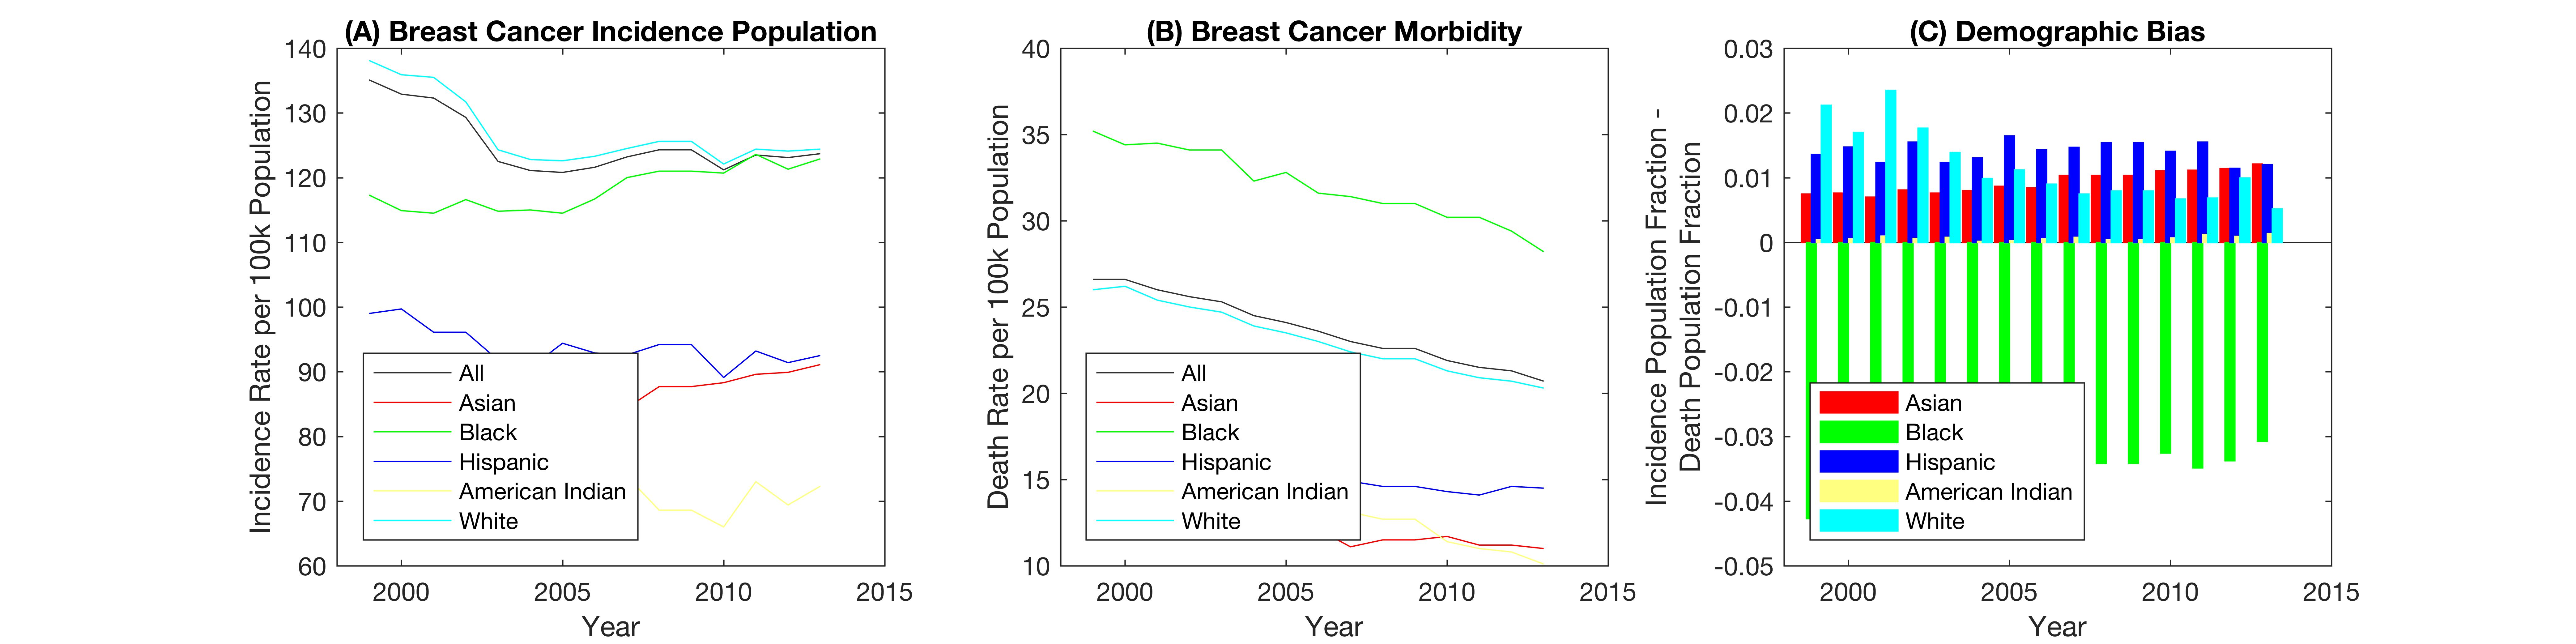
\includegraphics[width=1\columnwidth, trim = {20cm 0cm 10cm 0cm}, clip]{Figures/Rationale.jpg}
\caption{\label{PS} Rationale to investigate the representation of cell models derived from black patients in breast cancer research based on a persistent discrepancy in breast cancer treatment efficacy for black patients. }
\end{figure}

A success of the medical community is the morbidity for all patients has steadily decreased since 1999, figure 1B. Review of the CDC statistics exposes Black patients face the worst prognosis for survival on diagnosis. Black patients comprise more of the death population than the incidence, the incidence population fraction is less than the death population fraction, figure 1C. Black patients are less likely to survive than other races, exposing a well-acknowledged disparity in the efficacy of breast cancer treatment for black women \cite{greenlee2000cancer, berkman2014racial}. Surprisingly, when the fractions of each ethnicity in the incidence population are compared to the death population, black patient's fraction increase, meaning more black woman die after a breast cancer diagnosis than other ethnicities. Black patients comprise more of the death population than the incidence, the incidence population fraction is less than the death population fraction, figure 1C. White woman comprised the same 83\% of the death population as they did the incidence population, while  Asian, Hispanic and Native American fractions decrease slightly. From this we learn breast cancer treatment is less effective in treating blacks than all other races. 

Raising the survival rate of Black breast cancer patients to the national average requires critical review of societal, behavioral and biological factors, broadly categorized as extrinsic factors which are the responsibility of public policy and the individual, and intrinsic factors, such as genetics and cell structure within aggressive tumor sub-types, which are the responsibility of medical researchers to consider in designing fundamental research studies \cite{reding2012examination, brennan2012there}. Socioeconomic-dependence of high-quality health care access and inclusive diagnostic techniques, without question \cite{shavers2003racial}. Failing to diagnosis at early stages, as well as faster growing, more aggressive tumor sub-types, disproportionately effect black patients \cite{batina2013variation}. 

Why? Could this be due to access to medical care? Yes. Could this be due to bias in the medical research used to build the scientific expertise, therapies and patents employed in hospitals? Possibly, lets review breast cancer research tools and their representation in the publication record. 

One breast cancer research tool may hinder generalization of results. It is the cell model. Select biopsies from patients are cataloged, creating a bank of standards, enabling comparison of experimental results across time and labs. Since cell lines are derived from patients, the cell line carries unique genetic traits specific to the individual, which diminish the applicability of the results to other members of the same patient population. One way around this limitation is to grow the catalog of available cell lines, which has been an ongoing process since the first cell line in 1951. How the research community uses the available set of cell lines shapes how representative the research is and how well the treatment work across the patient population.  

When comparing the fraction of an ethnicity in the incidence population, death population, cell line bank and publication record, we expect the most prevalent ethnicity in the incidence and death population to be the same, as well as the same ethnicity to be the most prevalent donor to the cell lines, and those cell lines to be the most widely cited in publications. Which is true.  White patients represent 83\% of the incidence population, the same percentage of the death population, slightly less, but still a majority of the cell lines were donated by white patients, and more than 95\% of the citations of cell line citation in the publication record are of the cell lines donated by white patients. This is all logical. Research effort should reflect the greatest need, representing the majority of patients not receiving suitable treatment. However, as treatment are developed, effectively curing patients, let's refocus 

\begin{figure}[h!]
\centering
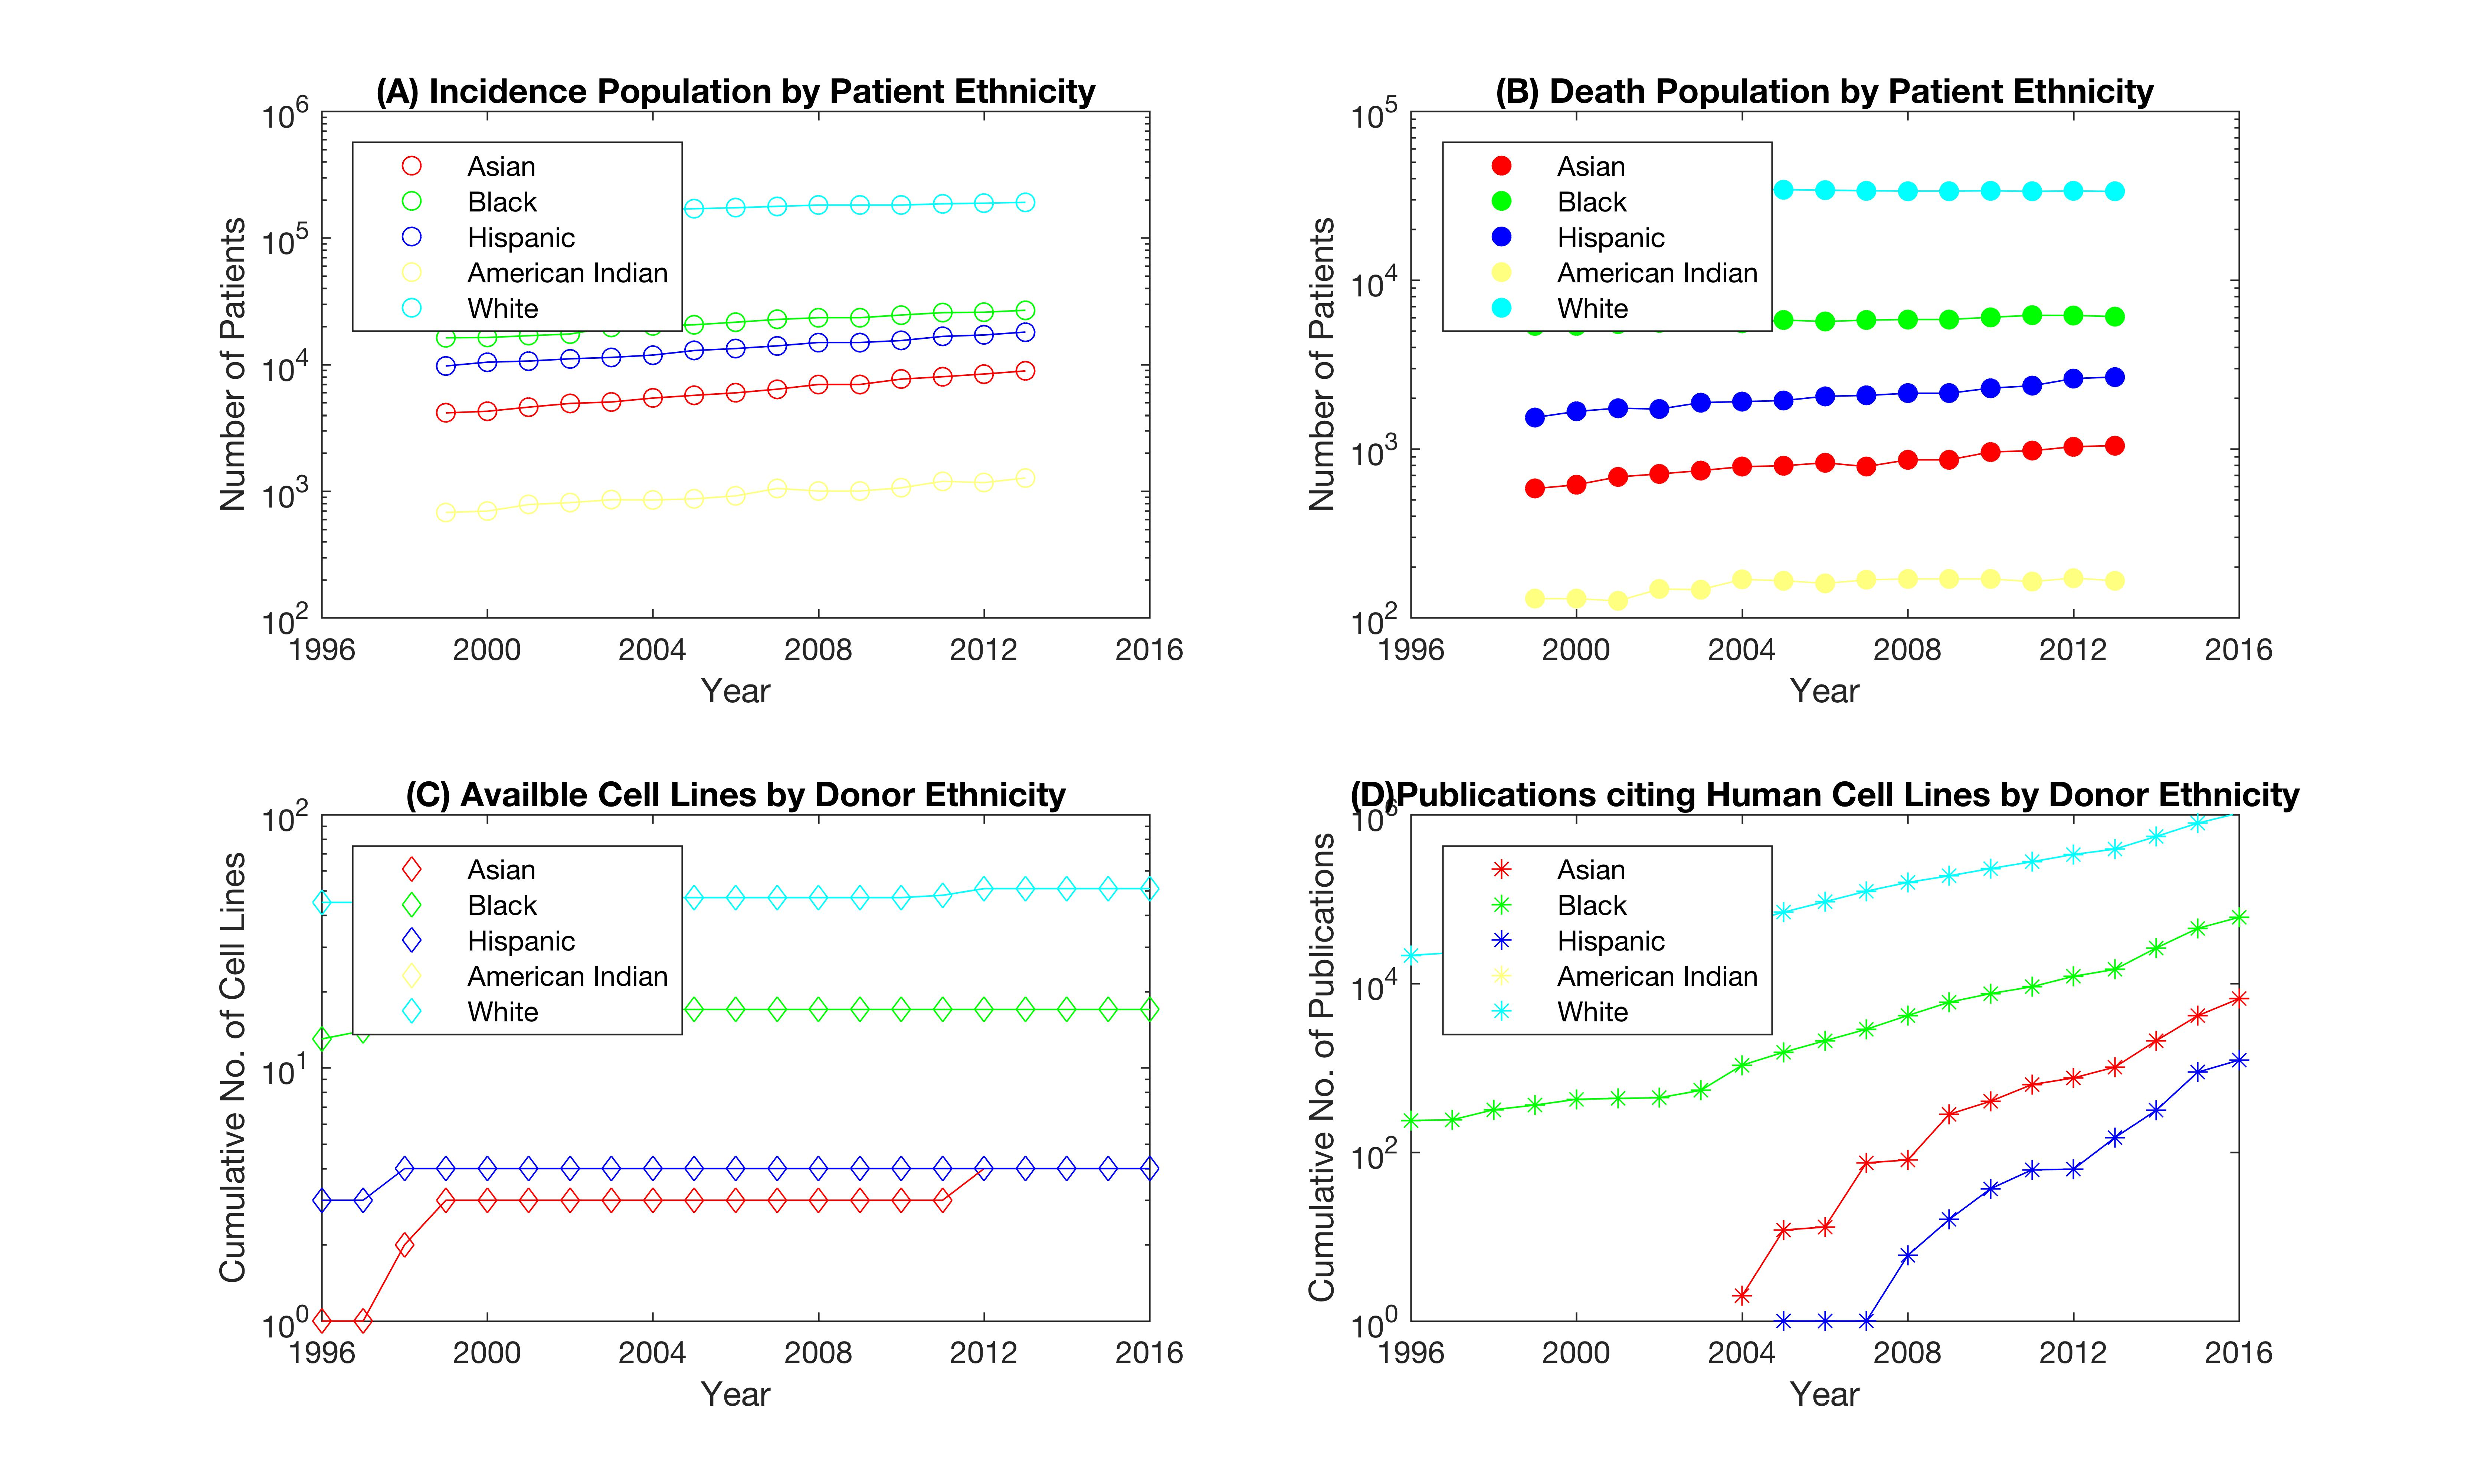
\includegraphics[width=1\columnwidth, trim = {10cm 0cm 10cm 0cm}, clip]{Figures/Timeline2x2.jpg}
\caption{\label{PS} Demographic representation in available cell lines, publication and patents as compared to the death counts for breast cancer.}
\end{figure}

The breast cancer patient population includes all ethnic groups. Sorting the fraction each ethnic group comprises of the incidence population lists the groups from most to least as White, Black, Hispanic, Asian and Native American, least populus, shown in figure 2A. Matching the trend, the death population shows the same list when sorted by fraction from most populus to least, figure 2B. 

Considering the finite resources available to the medical research community and their charge to provide care for the patient population, it is unsurprising the breast cancer cell line bank reflects the same representative bias as the incidence and death population, figure 2C. Of the 154 cell lines available, 50\%, 78 cell lines were formed from donors of unknown ethnicity. Of the breast cancer cell lines of known donor ethnicity, 51 from White donors, 17 from Black donors, 4 from Hispanic donors, 4 from Asian donors, and none from Native American donors. 

Understanding the  importance of standards, reproducibility and the legacy of scientific research, we expect a bias in the publication record towards a subset of the available cell lines, meaning cell lines donated by white patients will comprise a majority of the citation in publications, which is true. Of the more than 1.2 million publications citing a cell line, 1.0 million cited a cell line donated by a white patients, 60k cited a cell line donated by a black patient, 6k cited a cell line donated by an Asian patient, 1k cited a cell line donated by a Hispanic patient and none cited a cell line donated by a Native American patient, because there were no Native American cell line available, figure 2D.


How does the fraction of woman in the incidence population compare to the fraction of publication citing a breast cancer cell line donated by a white woman? Since 1999, the fraction of white woman has been less than the fraction of cell lines donated by white woman by more than 15\%, rising to nearly 19\% in 2013, figure 3A. In discussing fractions, if cellular material donated by White patients has been over represented compared to the patient population, the other ethnicites were under-represented by the same metric. Which is true. The under-representation of Hispanics increased from 3\% to nearly 6\% in 2013. The trend is exaggerated when comparing the death population fraction to the publication record. 

\begin{figure}[h!]
\centering
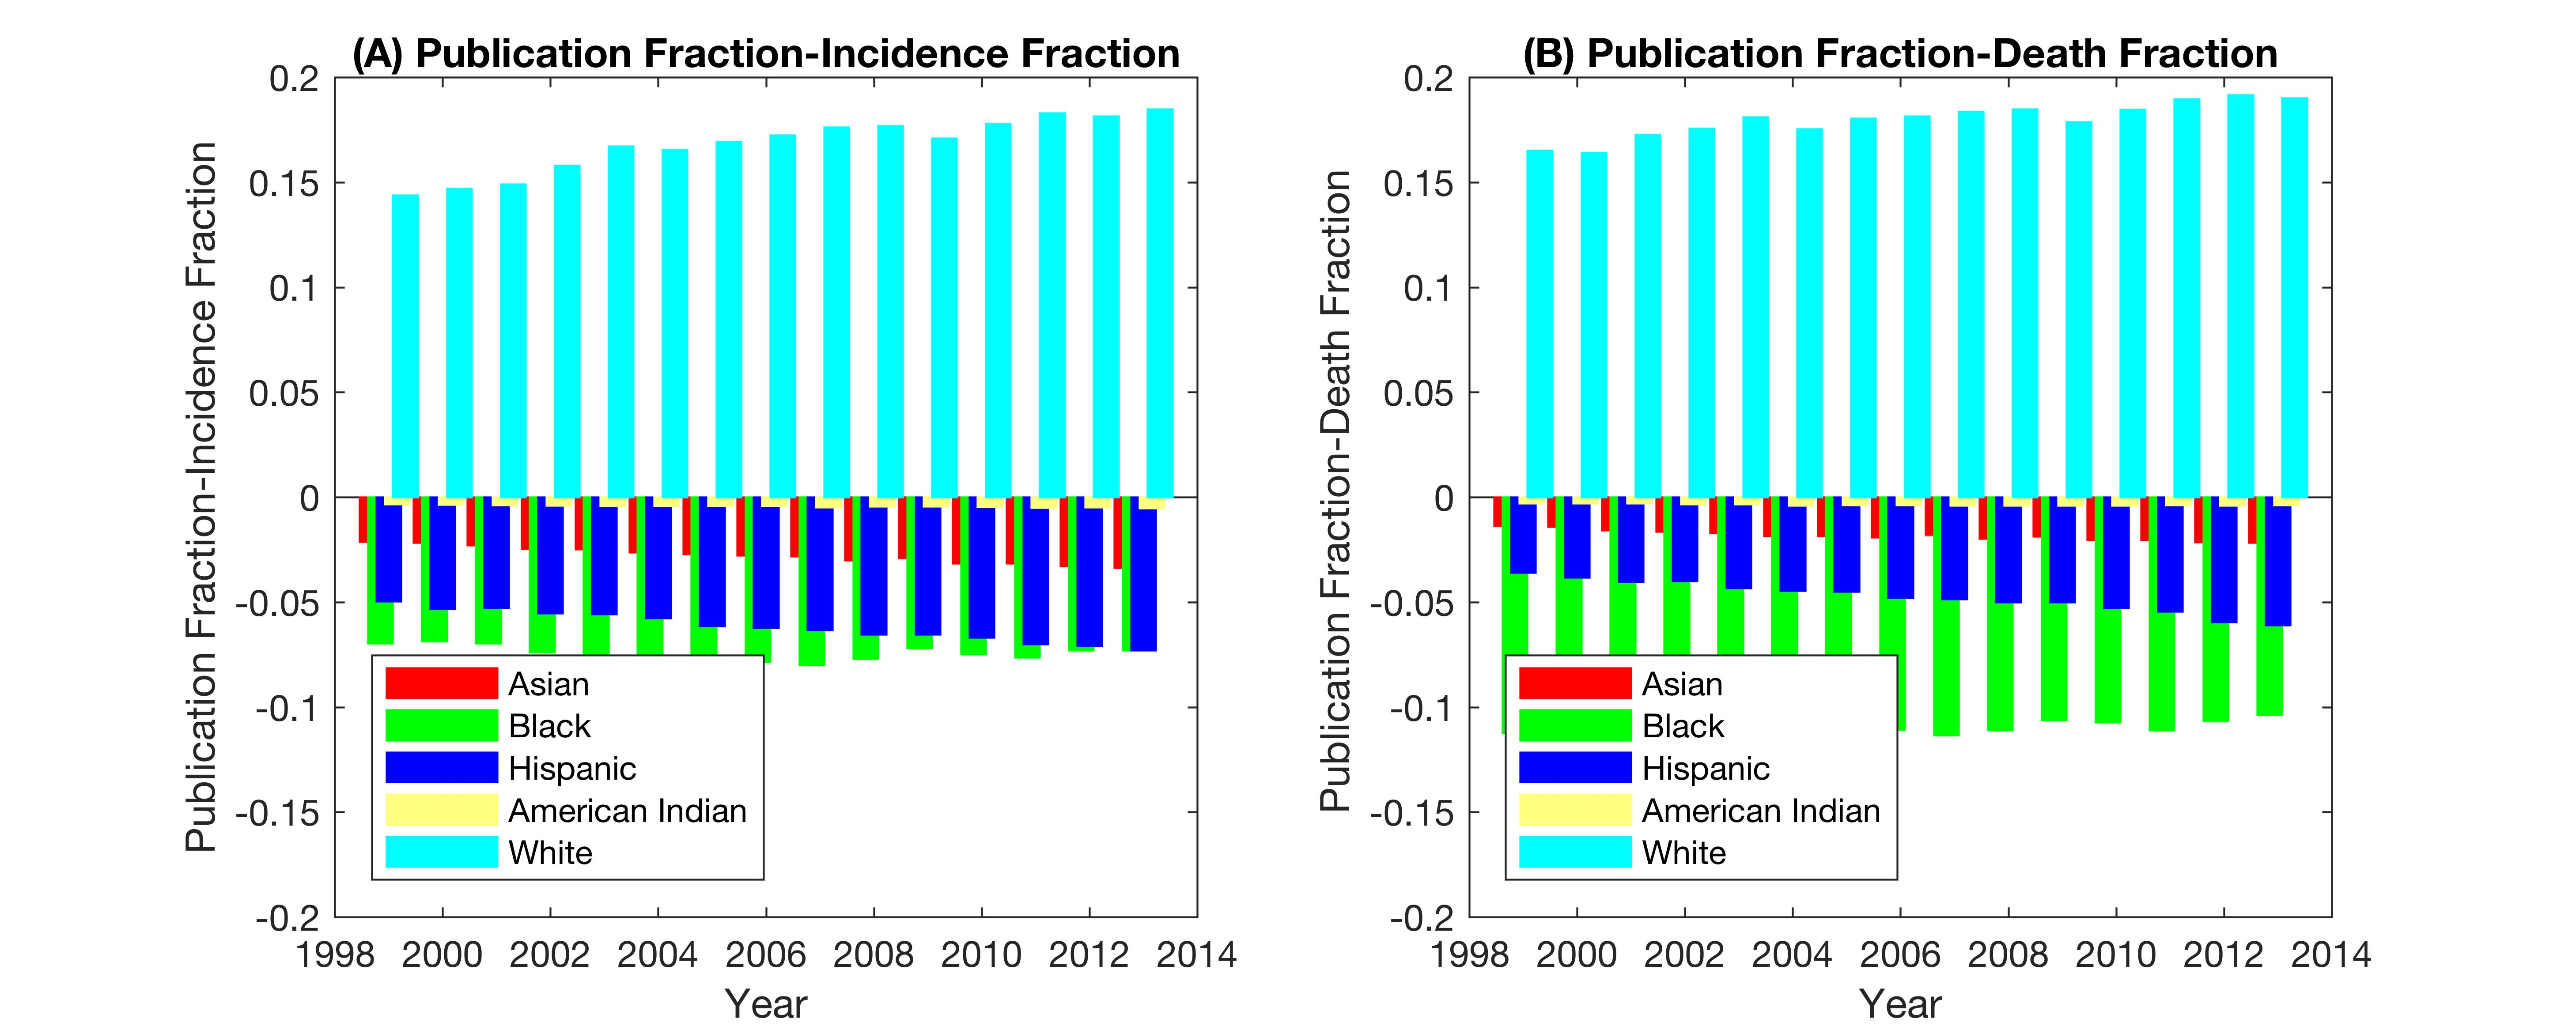
\includegraphics[width=1\columnwidth, trim = {10cm 0cm 10cm 0cm}, clip]{Figures/Bias.jpg}
\caption{\label{Bias} The representative bias in breast cancer medical research and therapeutic development, as determined by comparing the fraction of each demographic in the breast cancer death count to the number of publications and US patents citing cell lines generated from each ethnicity.}
\end{figure}

How would dependence on a subset of cell models influence the generalizability of medical results? Are there specific genetically sensitive targets which are prevalent in Black patients, which are not included in cell models donated by White patients? 

Research supports black breast cancer patients present elevated risk for aggressive, intrinsic factors of breast cancer which adversely effect prognosis. The next logical question is to what extent have black patients donated to cell lines used by medical researchers, and then, how well these lines are represented in published research and patents. The purpose of asking these questions is to determine any extent to under-representation, allowing for corrective action to simply include cell lines which represent the aggressive tumor sub-types causing the most morbidity. Data-driven retrospectives on disease burden and treatment effectiveness have been used in the past to guide medical research funding and health policy decisions towards the most productive population-level outcomes \cite{kim2016cancer}. 

The likely causes include societal, behavioral and biological factors, broadly categorized as extrinsic factors which are the responsibility of public policy and the individual, and intrinsic factors, such as genetics and cell structure within aggressive tumor sub-types, which are the responsibility of medical researchers to consider in designing fundamental research studies \cite{reding2012examination, brennan2012there}. 

Raising the survival rate of black breast cancer patients to the national average requires critical review of socioeconomic-dependence of high-quality health care access and inclusive diagnostic techniques, without question \cite{shavers2003racial}. Failing to diagnosis at early stages, as well as faster growing, more aggressive tumor sub-types, disproportionately effect black patients \cite{batina2013variation}. 

Vetting the influence of intrinsic factors of breast cancer is critical to guide the action of fundamental medical research, especially the types of cell lines used in foundational research. Are there intrinsic factors of the tumor sub-types causing morbidity, which are disproportionately present in in black breast cancer patients? Environmental exposure and genetic background determine the breast cancer's subtypes, aggressiveness, and ultimately, patient's prognosis. Highly aggressive tumor subtypes are correlated to risk factors such as obesity, which disproportionately effects black women. Self-reported race correlated to breast cancer properties, such as estrogen receptor status and stage of diagnosis, more than percent African ancestry, suggesting social determinants shape the disease physiology more than genetic predispositions \cite{reding2012examination}. Currently, alternative treatment options for patients with a genetic predisposition for hormone receptor-negative breast cancers, which are also likely black, is  limited \cite{huo2009population}.

Research supports black breast cancer patients present elevated risk for aggressive, intrinsic factors of breast cancer which adversely effect prognosis. The next logical question is to what extent have black patients donated to cell lines used by medical researchers, and then, how well these lines are represented in published research and patents. The purpose of asking these questions is to determine any extent to under-representation, allowing for corrective action to simply include cell lines which represent the aggressive tumor sub-types causing the most morbidity. Data-driven retrospectives on disease burden and treatment effectiveness have been used in the past to guide medical research funding and health policy decisions towards the most productive population-level outcomes \cite{kim2016cancer}. 

The long term consequences of medical research in demographics most heavily represented as donors to biopsies used in lab work have the best prognosis for treatment. Targeted breast cancer therapies and preventative screening sensitive to various tumors are required to absolve demographic inequalities in breast cancer treatment \cite{batina2013variation}. Cell lines are a critical tool of scientific discovery for medical treatments. ``Human cancer in a test tube'' provides a standard for genotypic and phenotypic stability. 

The next steps in breast cancer research characterizes the many sub-types of breast cancer as unique pathologies, relying on specific traits of the tumor and the patient's genetics to make decisions regarding treatment options. As the medical community pivots towards personalizing care based on genetic markers, we reflect on the inertia of breast cancer research. After acknowledging new genomic techniques change how we group patients, lets consider past use of ethnic groups. Before gene sequencing became widely available, the CDC grouped the US breast cancer patient population by ethnicity, to identify if and who was left out of improving health care options. The purpose being to expand healthy lifestyle choices, public awareness campaigns, diagnostics, and treatment options to include non-majority considerations. Cell model breast cancer research has developed tool to study non-majority ethnicities in the patient population, with the notable exception of Native Americans. Reliance on a select subset of these tool as standards to study breast cancer perpetuated the bias. An emphasis on genetics and tumor sub-types offers the possibility to refine the vocabulary used to group breast cancer patients, targeting differences in disease treatment option are able to directly address. 

\bibliographystyle{unsrt}
\bibliography{refs}


\end{document}